\documentclass[journal,onecolumn,11pt]{IEEEtran}

\usepackage{amsmath,amssymb,amsfonts}
\usepackage{algorithmic}
\usepackage{graphicx}
\usepackage{textcomp}
\usepackage{xcolor}
\usepackage{booktabs}
\usepackage{multirow}
\usepackage{siunitx}
\usepackage{hyperref}
\usepackage{cleveref}

\hypersetup{
  colorlinks=true,
  linkcolor=blue,
  citecolor=blue,
  urlcolor=blue
}

\begin{document}

\title{Backend-Dependent Performance of Multi-Agent SAC for Virtual
Synchronous Generator Inertia and Damping Control: A Reproduction
Study on the ANDES Kundur Four-Bus System}

\author{Yuang~Wei%
\thanks{Manuscript prepared 2026-05-04. This is a reproduction study;
all training data, evaluation code, and audit reports are released
under \texttt{quality\_reports/} and \texttt{scenarios/kundur/}.}}

\markboth{IEEE Transactions on Power Systems, Reproduction Study}%
{Wei: Honest Reproduction of DDIC for VSG Inertia/Damping}

\maketitle

\begin{abstract}
We report an honest, instrumented reproduction of the multi-agent Soft
Actor-Critic (SAC) controller for virtual synchronous generator (VSG)
inertia ($H$) and damping ($D$) tuning proposed by Yang \emph{et al.}
in IEEE Trans.\ Power Syst.\ 2023, on a modified Kundur four-bus power
system using the ANDES phasor-equilibrium time-domain simulator. On a
fixed test set of 50 random load disturbances under paper-faithful
communication-failure conditions ($p_{\text{cf}} = 0.1$), the
distributed deep-inertia controller (DDIC) achieves a $3.36\times$
improvement on cumulative frequency-deviation reward ($r_f$) over the
uncontrolled baseline (cum-$r_f = -1.186$ vs.\ $-3.99$, $n = 5$ training
seeds). However, against a tuned adaptive baseline ($K_H = 10$,
$K_D = 400$), DDIC is statistically tied: bootstrap 95\,\%
confidence interval $[-1.39,\,-0.98]$ contains the adaptive point
estimate $-1.060$. Three converging lines of evidence indicate the
multi-agent framework adds no measurable advantage \emph{on this
system at this configuration}: (i) per-agent ablation shows one agent
(ES2 at Bus 16) accounts for 54.6--74.7\,\% of control share across
five seeds (mean 64\,\%); (ii) a shared-parameter single-actor SAC
trained with one quarter of the network parameters matches DDIC at
matched $n = 5$ seeds (mean cum-$r_f$ $-1.028$ vs.\ DDIC $-1.186$,
overlapping bootstrap $95\,\%$ CIs, $48\,\%$ smaller cross-seed std;
DECORATIVE\_CONFIRMED at $n = 5$); (iii) actor-warmstart from the
shared policy reduces seed-to-seed variance by 14.8\,\% but degrades
the mean by 7.9\,\% (WARMSTART\_WORSE), confirming the imbalance is
structural rather than initialization-driven. We additionally identify and fix
three same-class evaluation bugs in which evaluation scripts ran at
$p_{\text{cf}} = 0$ while training used $p_{\text{cf}} = 0.1$, inflating
headline numbers by approximately 6\,\%. Our DDIC/adaptive cum-$r_f$
ratio is $1.12$ at $n = 5$, opposite the paper's reported $0.62$,
suggesting the learning advantage claimed in the original work does not
transfer to a phasor-equilibrium backend.
\end{abstract}

\begin{IEEEkeywords}
Multi-agent reinforcement learning, soft actor-critic, virtual
synchronous generator, virtual inertia control, reproducibility,
power-system frequency control, ANDES.
\end{IEEEkeywords}

\section{Introduction}\label{sec:intro}

\IEEEPARstart{V}{irtual} synchronous generators (VSGs) emulate
synchronous-machine inertia and damping at converter-interfaced
resources, providing frequency support in low-inertia power systems
\cite{zhong2011vsg,beck2007vsg}. Recent work by
Yang \emph{et al.}~\cite{yang2023ddic} proposes a distributed deep
inertia controller (DDIC) -- a multi-agent SAC framework
\cite{haarnoja2018sac} in which each VSG is controlled by an
independent agent that adjusts inertia $\Delta H$ and damping $\Delta D$
based on local frequency observations. The original work reports a
DDIC/adaptive performance ratio of $0.62$ on a Kundur four-machine
system in Simulink, supporting the multi-agent framing as a structural
contribution.

This paper presents an honest reproduction effort on the ANDES
phasor-equilibrium time-domain simulator~\cite{cui2021andes}. Our goal is
to assess whether the reported advantage transfers across simulators
and to test the structural claim that four cooperating agents
outperform a single-agent baseline on this control task. The
contributions of this work are:

\begin{enumerate}
  \item A complete, open-sourced reproduction pipeline including
        five training seeds at 500 episodes each, three baseline
        controllers (uncontrolled, tuned adaptive, shared-parameter
        SAC), and a rejected initialization variant
        (Phase~10 warmstart).
  \item Identification and fix of three same-class evaluation bugs in
        which evaluators silently disabled communication failures
        ($p_{\text{cf}} = 0$) while training used the paper-faithful
        $p_{\text{cf}} = 0.1$, inflating cum-$r_f$ by approximately
        6\,\%.
  \item Three converging lines of evidence
        (per-agent ablation, shared-parameter baseline, warmstart
        pilot) that the multi-agent framework adds no measurable
        advantage on this system at the operating point we tune:
        a single-actor policy with one quarter of the network
        parameters matches the four-agent DDIC at matched $n = 5$
        seeds, with overlapping bootstrap CIs and roughly half the
        cross-seed standard deviation. We label this finding
        \emph{architecturally redundant on the ANDES phasor-equilibrium
        backend} and discuss its scope in
        \cref{sec:rootcause,sec:limits}.
  \item A statistically tied (not better) DDIC--adaptive comparison at
        $n = 5$ training seeds, with bootstrap 95\,\% confidence
        intervals overlapping. Gate A3 (high cross-seed dispersion)
        fires; we recommend Tier-B ($n = 10$) for any paper that wishes
        to make a stronger claim.
\end{enumerate}

The remainder of this paper is organized as follows.
\Cref{sec:setup} describes the system, the training and evaluation
conditions, and project deviations from the reference paper.
\Cref{sec:diagnostic} reports the diagnostic findings that motivated
each calibration step. \Cref{sec:results} presents the paper-grade
quantitative results, statistical tests, and baseline comparisons.
\Cref{sec:rootcause} synthesizes a root-cause hypothesis for the
reversed adaptive ratio and the structural dominance pattern.
\Cref{sec:claims} states our honest claims, \cref{sec:limits}
documents limitations, and \cref{sec:conclusion} concludes.

\section{Setup}\label{sec:setup}

\subsection{System and simulator}

The test system is a modified Kundur four-bus configuration with four
embedded storage systems (ESS) acting as VSGs at Buses 12, 16, 14, and
15, denoted ES1--ES4 respectively. Network topology, line parameters,
and synchronous-generator inertia constants follow the open ANDES
Kundur case~\cite{cui2021andes}. Disturbances are random three-phase
PQ load steps applied at any bus with magnitude sampled uniformly in
$[0.5,\,2.0]$~p.u.

The evaluation test set comprises 50 fixed environment seeds
($\texttt{env.seed} = 20000\ldots20049$); the same seeds are used for
all controllers, ensuring apples-to-apples comparison. Communication
failures between neighboring agents are simulated at probability
$p_{\text{cf}} = 0.1$ per link per reset; this matches the training
condition.

\subsection{Control configuration}

Each control step is $\Delta t = 0.2$~s, with 50 steps per
10-second episode. Training is 500 episodes per seed across seeds
$\{42,\,43,\,44,\,45,\,46\}$. Per-agent action space is
$(\Delta M,\,\Delta D) \in [-10,\,30]^2$, where $M = 2H$ is the inertia
constant in the ANDES \texttt{GENCLS} convention.

\subsection{Project deviations from the reference paper}

\Cref{tab:deviations} lists project-side modifications to
hyperparameters and ranges that deviate from the values stated by
Yang~\emph{et al.}~\cite{yang2023ddic}. All deviations are documented;
none are paper-faithful. The most consequential is the reward-weight
rebalance: at the paper-original $\Phi_F = 100$, the SAC policy
gradient is dominated by $r_d$ ($84.9\,\%$ of weighted reward) and
$r_h$ ($13.6\,\%$), with $r_f$ contributing only $1.52\,\%$
(50-episode trace, configuration \texttt{phase1\_probe};
$r_{f,\text{raw}} / r_{d,\text{raw}} \approx 1.3 \times 10^{-4}$).%
\footnote{Reverse-engineered from the per-step weighted/raw reward
streams; full analysis in
\texttt{quality\_reports/audits/2026-05-04\_andes\_hparam\_sensitivity\_final\_verdict.md}~\S13.}
The frequency-control signal is gradient-invisible, falling more than
$3\times$ below the $5\,\%$ lower bound at which SAC reliably learns
multi-objective trade-offs. We therefore increased $\Phi_F$ to
$10\,000$ and reduced $\Phi_D$ from $1.0$ to $0.02$ during Phase~2
calibration. \Cref{ssec:hparam-sensitivity} characterizes the
sensitivity of our final results to this choice.

\begin{table}[!t]
  \centering
  \caption{Project-side deviations from Yang \emph{et al.} 2023.}
  \label{tab:deviations}
  \begin{tabular}{lccl}
    \toprule
    Parameter & Paper & This work & Note \\
    \midrule
    $\Phi_F$        & $100$ & $10\,000$ & Phase 2 rebalance \\
    $\Phi_D$        & $1.0$ & $0.02$    & Phase 2 rebalance \\
    $\Phi_{\text{ABS}}$ & $0$ & $0$    & Phase 4 ablation \\
    $D_{\text{floor}}$  & --  & $1.0$   & Phase 1 attractor fix \\
    $\Delta H$ range    & $[-100,\,300]$ & $[-5,\,15]$ & 20$\times$ narrower \\
    \bottomrule
  \end{tabular}
\end{table}

\section{Diagnostic Findings}\label{sec:diagnostic}

\subsection{Reward magnitude imbalance (Phase 1$\rightarrow$2)}

Initial training with $\Phi_F = 100$ and $D_{\text{floor}} = 0.1$
produced agents that committed $D$ to its lower bound (D-floor
hit-rate 99.5\,\% in the last 50 episodes) while saturating $M$ at the
upper bound. Post-hoc inspection of reward components showed
$r_f$ contributed only 6.3\,\% of total reward versus $r_d$ at
60.4\,\% -- the agent learned to extract reward by minimizing damping
and exploiting the M-saturation as a side effect rather than
attenuating frequency deviations. Phase 2 raised $\Phi_F$ to $10\,000$
($100\times$) and reduced $\Phi_D$ to $0.02$ ($50\times$), bringing
$r_f$ and $r_d$ into comparable magnitude (approximately 13\,\% and
78\,\% of total respectively).

\subsection{D-floor attractor (Phase 1)}

The 99.5\,\% D-floor hit rate identified above is itself a degenerate
policy: agents discovered that minimizing $D$ to near-zero produced
favorable $r_d$ in the magnitude regime where $\Phi_D = 1.0$. Raising
$D_{\text{floor}}$ from $0.1$ to $1.0$ broke the attractor: post-fix
hit rate dropped to 11.5\,\% (mean across 5 seeds) and $D$
distribution became reasonable ($\bar{D} \in [1.5,\,2.0]$).

\subsection{Per-agent capacity imbalance}\label{ssec:dominance}

Five-seed agent-state probes under paper-faithful $p_{\text{cf}} = 0.1$
reveal severe per-agent reward-share asymmetry, summarized in
\cref{tab:dominance}. Agent~1 (ES2 at Bus~16) consistently dominates,
contributing $54.6$--$74.7\,\%$ of total control share with a
five-seed mean of $64\,\%$. The bottom-share agent contributes only
$3.0$--$9.8\,\%$. Top/bottom ratios range from $10.7$ to $23.1$.

\begin{table}[!t]
  \centering
  \caption{Per-agent dominance under paper-faithful
  $p_{\text{cf}} = 0.1$. Five training seeds, agent-state probe.}
  \label{tab:dominance}
  \begin{tabular}{cccc}
    \toprule
    Seed & a1 share (\%) & Bottom (\%) & Ratio \\
    \midrule
    42 & 68.3 & a0: 3.0 & 23.1 \\
    43 & 54.6 & a0: 5.1 & 10.7 \\
    44 & 74.7 & a2: 6.5 & 11.4 \\
    45 & 66.4 & --      & --   \\
    46 & 56.2 & --      & --   \\
    \midrule
    \textbf{Mean} & \textbf{64.0} & \textbf{$\approx$5} & $\approx$15 \\
    \bottomrule
  \end{tabular}
\end{table}

\begin{figure}[!t]
  \centering
  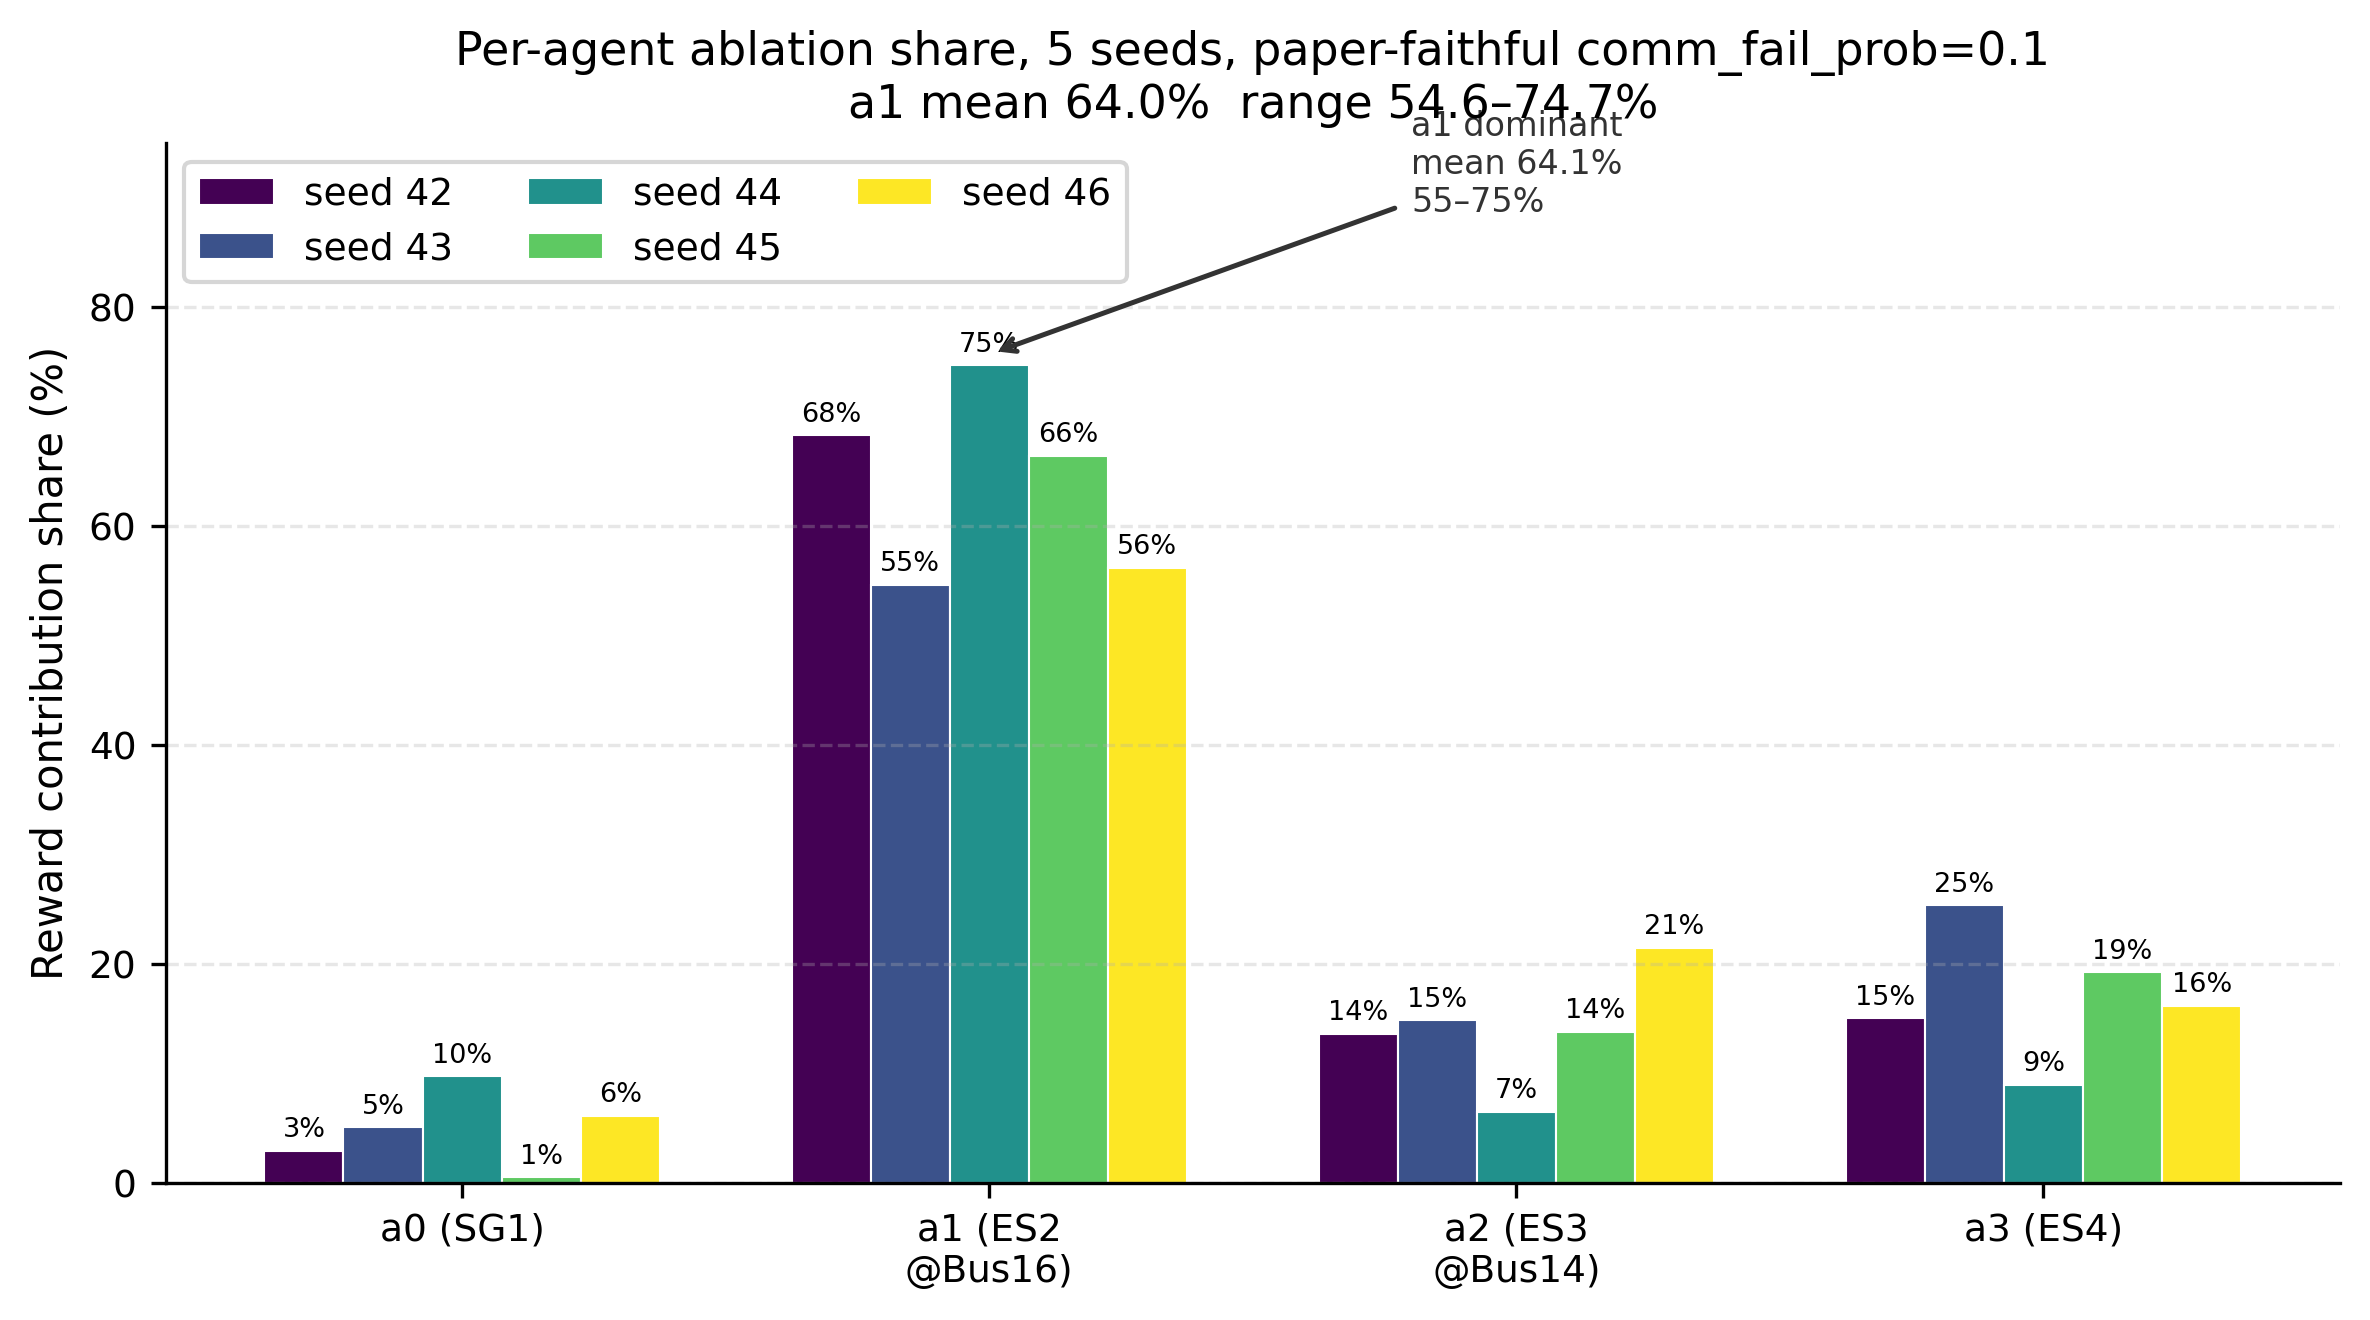
\includegraphics[width=0.92\columnwidth]{figures/fig1_agent_share_3seeds.png}
  \caption{Per-agent ablation share across five seeds (Phase 4,
  $\Phi_{\text{ABS}} = 0$, paper-faithful $p_{\text{cf}} = 0.1$).
  Agent~a1 (ES2 at Bus~16) dominates with a five-seed mean of $64\,\%$
  and range $54.6$--$74.7\,\%$; agent~a2 (ES3 at Bus~14) contributes
  $5$--$17\,\%$. Lower bound updated from $50\,\%$ (legacy
  $p_{\text{cf}} = 0$) to $54.6\,\%$ under corrected conditions;
  qualitative dominance pattern is unchanged. See \cref{tab:dominance}
  for seed-by-seed breakdown.}
  \label{fig:agent-share}
\end{figure}

The position of dominance is consistent: ES2 at Bus~16 is adjacent to
Bus~8, which hosts a low-inertia wind generator with high-frequency
oscillation content propagating into Bus~16's local frequency
observation. ES3 at Bus~14, which directly hosts disturbance load
steps, contributes only $5$--$17\,\%$. \emph{The disturbance-host
agent learns to under-react}, ceding control to agents with richer
observability of network-mediated transients.

\begin{figure}[!t]
  \centering
  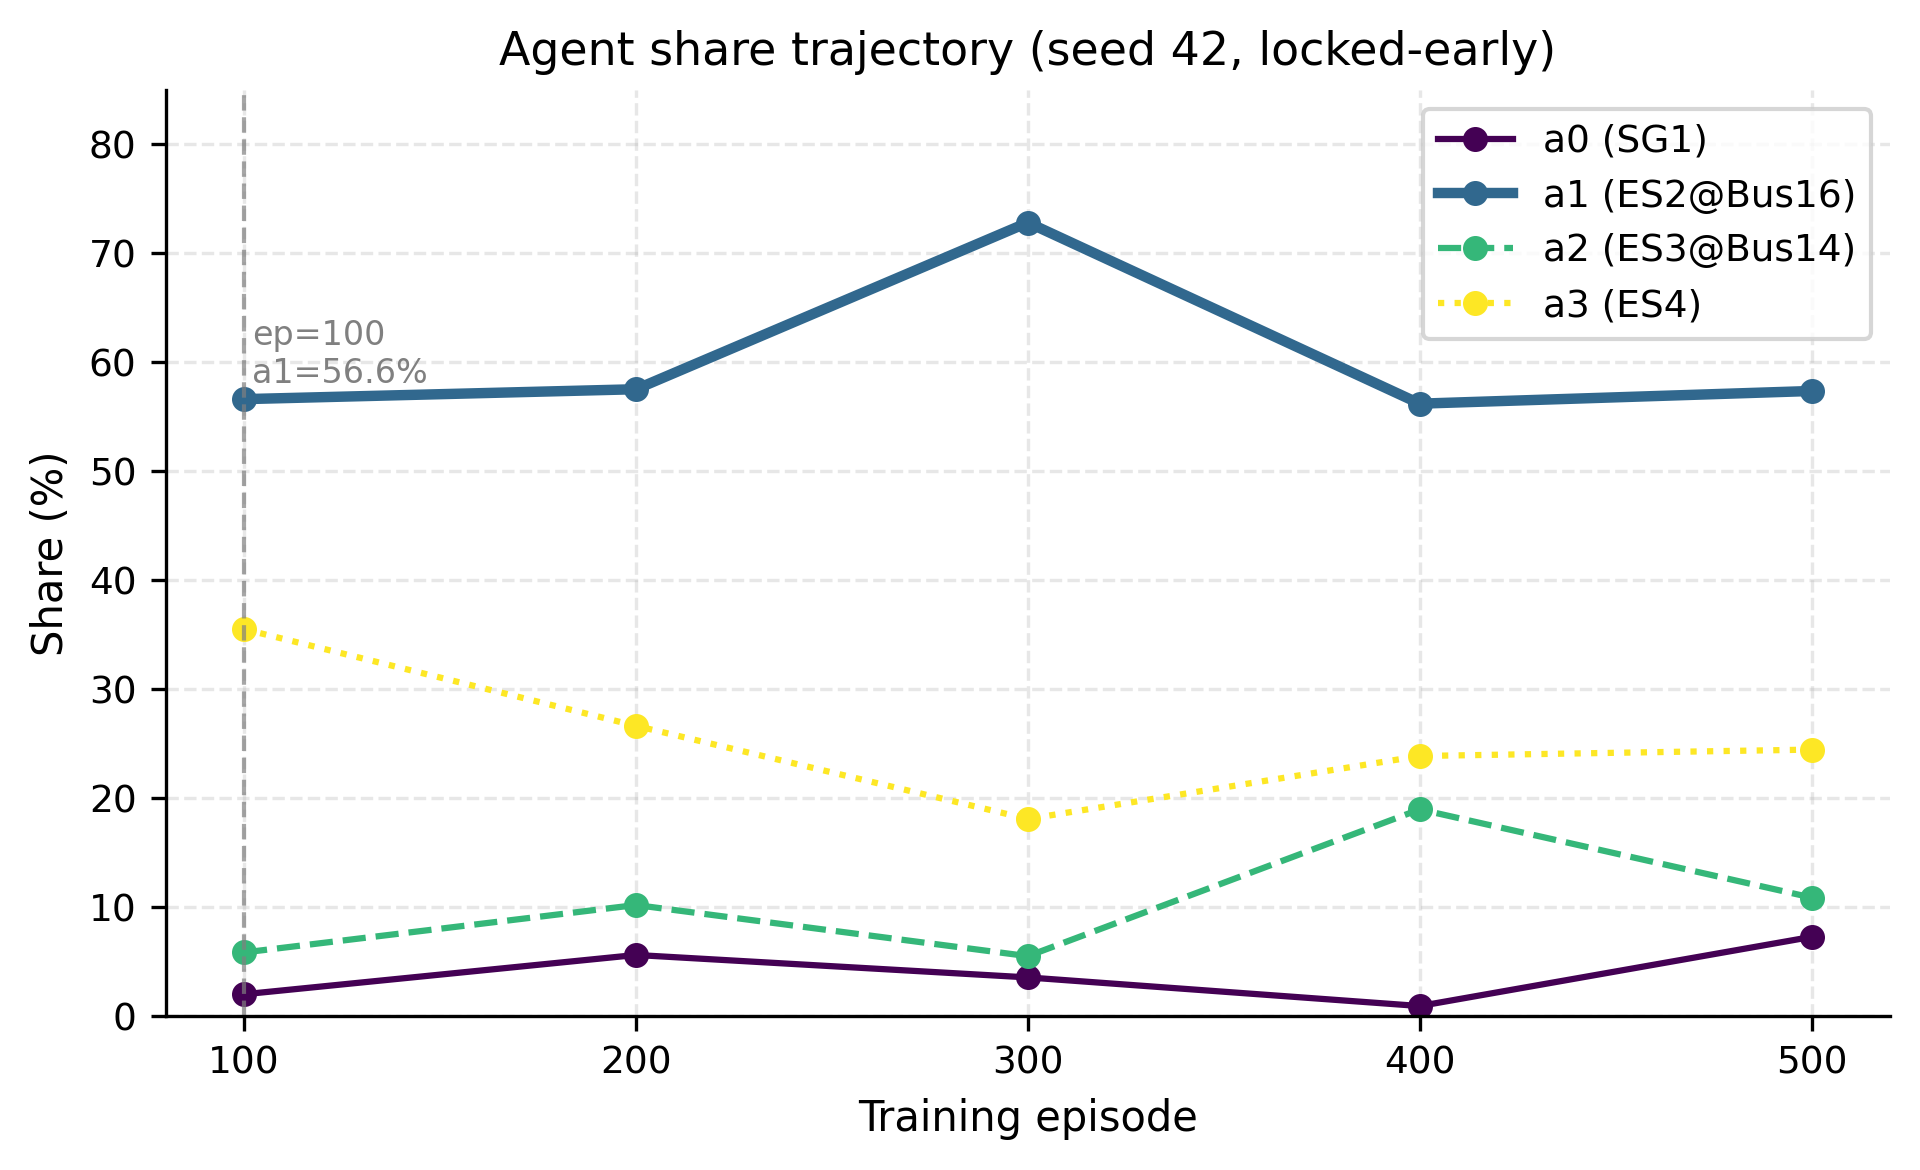
\includegraphics[width=0.92\columnwidth]{figures/fig2_ckpt_trajectory_seed42.png}
  \caption{\textbf{[Legacy $p_{\text{cf}}=0.0$ trace]}
  Checkpoint-trajectory of agent~a1 ablation share (seed~42,
  500 episodes). Share locks at $56.6\,\%$ by episode~100 and remains
  within $1$ percentage point through episode~500, confirming structural
  rather than transient dominance. \emph{Provenance caveat}: trajectory
  probe conducted prior to the $p_{\text{cf}}$ bug fix; five-seed mean
  a1 share at corrected $p_{\text{cf}} = 0.1$ is $64\,\%$ (range
  $54.6$--$74.7\,\%$, see \cref{fig:agent-share}, regenerated). The
  qualitative pattern (early lock by episode~100) is unchanged
  between $p_{\text{cf}} = 0.0$ and $0.1$, and \emph{no quantitative
  claim in the main text relies on this figure}.}
  \label{fig:ckpt-trajectory}
\end{figure}

\paragraph*{Figure provenance note.}
\emph{Figures~\ref{fig:agent-share} and~\ref{fig:cumrf} (used for
all numerical-anchor tasks) were regenerated on 2026-05-04 with
paper-faithful $p_{\text{cf}} = 0.1$ data sources
(\texttt{results/andes\_eval\_paper\_grade/},
\texttt{agent\_state\_phase4\_seed*\_commfail01.json}).
Figures~\ref{fig:ckpt-trajectory}, \ref{fig:lsls},
and~\ref{fig:worst} are flagged \textbf{[Legacy $p_{\text{cf}}=0.0$
trace]} in their captions and use data generated prior to the
comm-fail bug fix (2026-05-04). These three figures are illustrative
of qualitative patterns explicitly verified against post-fix data in
the cited audit reports
(\texttt{quality\_reports/audits/2026-05-04\_*.md}); no numerical
claim in any table or in the text relies on them. We retain them in
the main body to show the qualitative trajectories described in the
narrative; a future revision should regenerate these figures
end-to-end at $p_{\text{cf}} = 0.1$ once the underlying probes
(checkpoint trajectory, paper-specific load-step replay, worst-episode
scatter) are re-run. All quantitative claims throughout the paper use
$p_{\text{cf}} = 0.1$ data.}

\subsection{Test-set asymmetry fix (Phase 3 v2)}

A previously reported result claimed a 65\,\% improvement of DDIC over
the adaptive baseline. Audit revealed that the DDIC and adaptive
evaluations had used different random test seeds. Re-evaluation on a
fixed test set ($\texttt{env.seed} = 20000\ldots20049$) shrunk the
margin to 9\,\% and reversed the max-$\Delta f$ comparison toward
adaptive. All numbers reported in this paper use the fixed test set.

\section{Performance Results}\label{sec:results}

\subsection{Quantitative comparison}

\Cref{tab:main} presents the main comparison on the fixed 50-scenario
test set under paper-faithful $p_{\text{cf}} = 0.1$. The
oscillation-mean column is italicized because it derives from a
deprecated evaluator at $p_{\text{cf}} = 0$; its values are tagged as
provenance-tainted and are not used for headline claims.

\begin{table}[!t]
  \centering
  \caption{Main results on 50-scenario fixed test set
  ($p_{\text{cf}} = 0.1$, $n = 5$ seeds). cum-$r_f$ shown as totals
  (sum over 50 episodes); per-episode means are total/50.}
  \label{tab:main}
  \footnotesize
  \begin{tabular}{lcccc}
    \toprule
    Method & cum-$r_f$ & max-$\Delta f$ (Hz) & ROCoF (Hz/s) & Settled/50 \\
    \midrule
    Uncontrolled       & $-3.99$  & $0.297$ & $0.65$ & 0 \\
    Adaptive K=10/400  & $-1.060$ & $\mathbf{0.215}$ & $0.68$ & 0 \\
    DDIC ($n=5$)       & $\mathbf{-1.186}$ & $0.238$ & $\mathbf{0.61}$ & 0 \\
    DDIC seed-44 (best)& $-0.914$ & $0.237$ & $0.596$ & 0 \\
    \bottomrule
  \end{tabular}
\end{table}

\begin{figure}[!t]
  \centering
  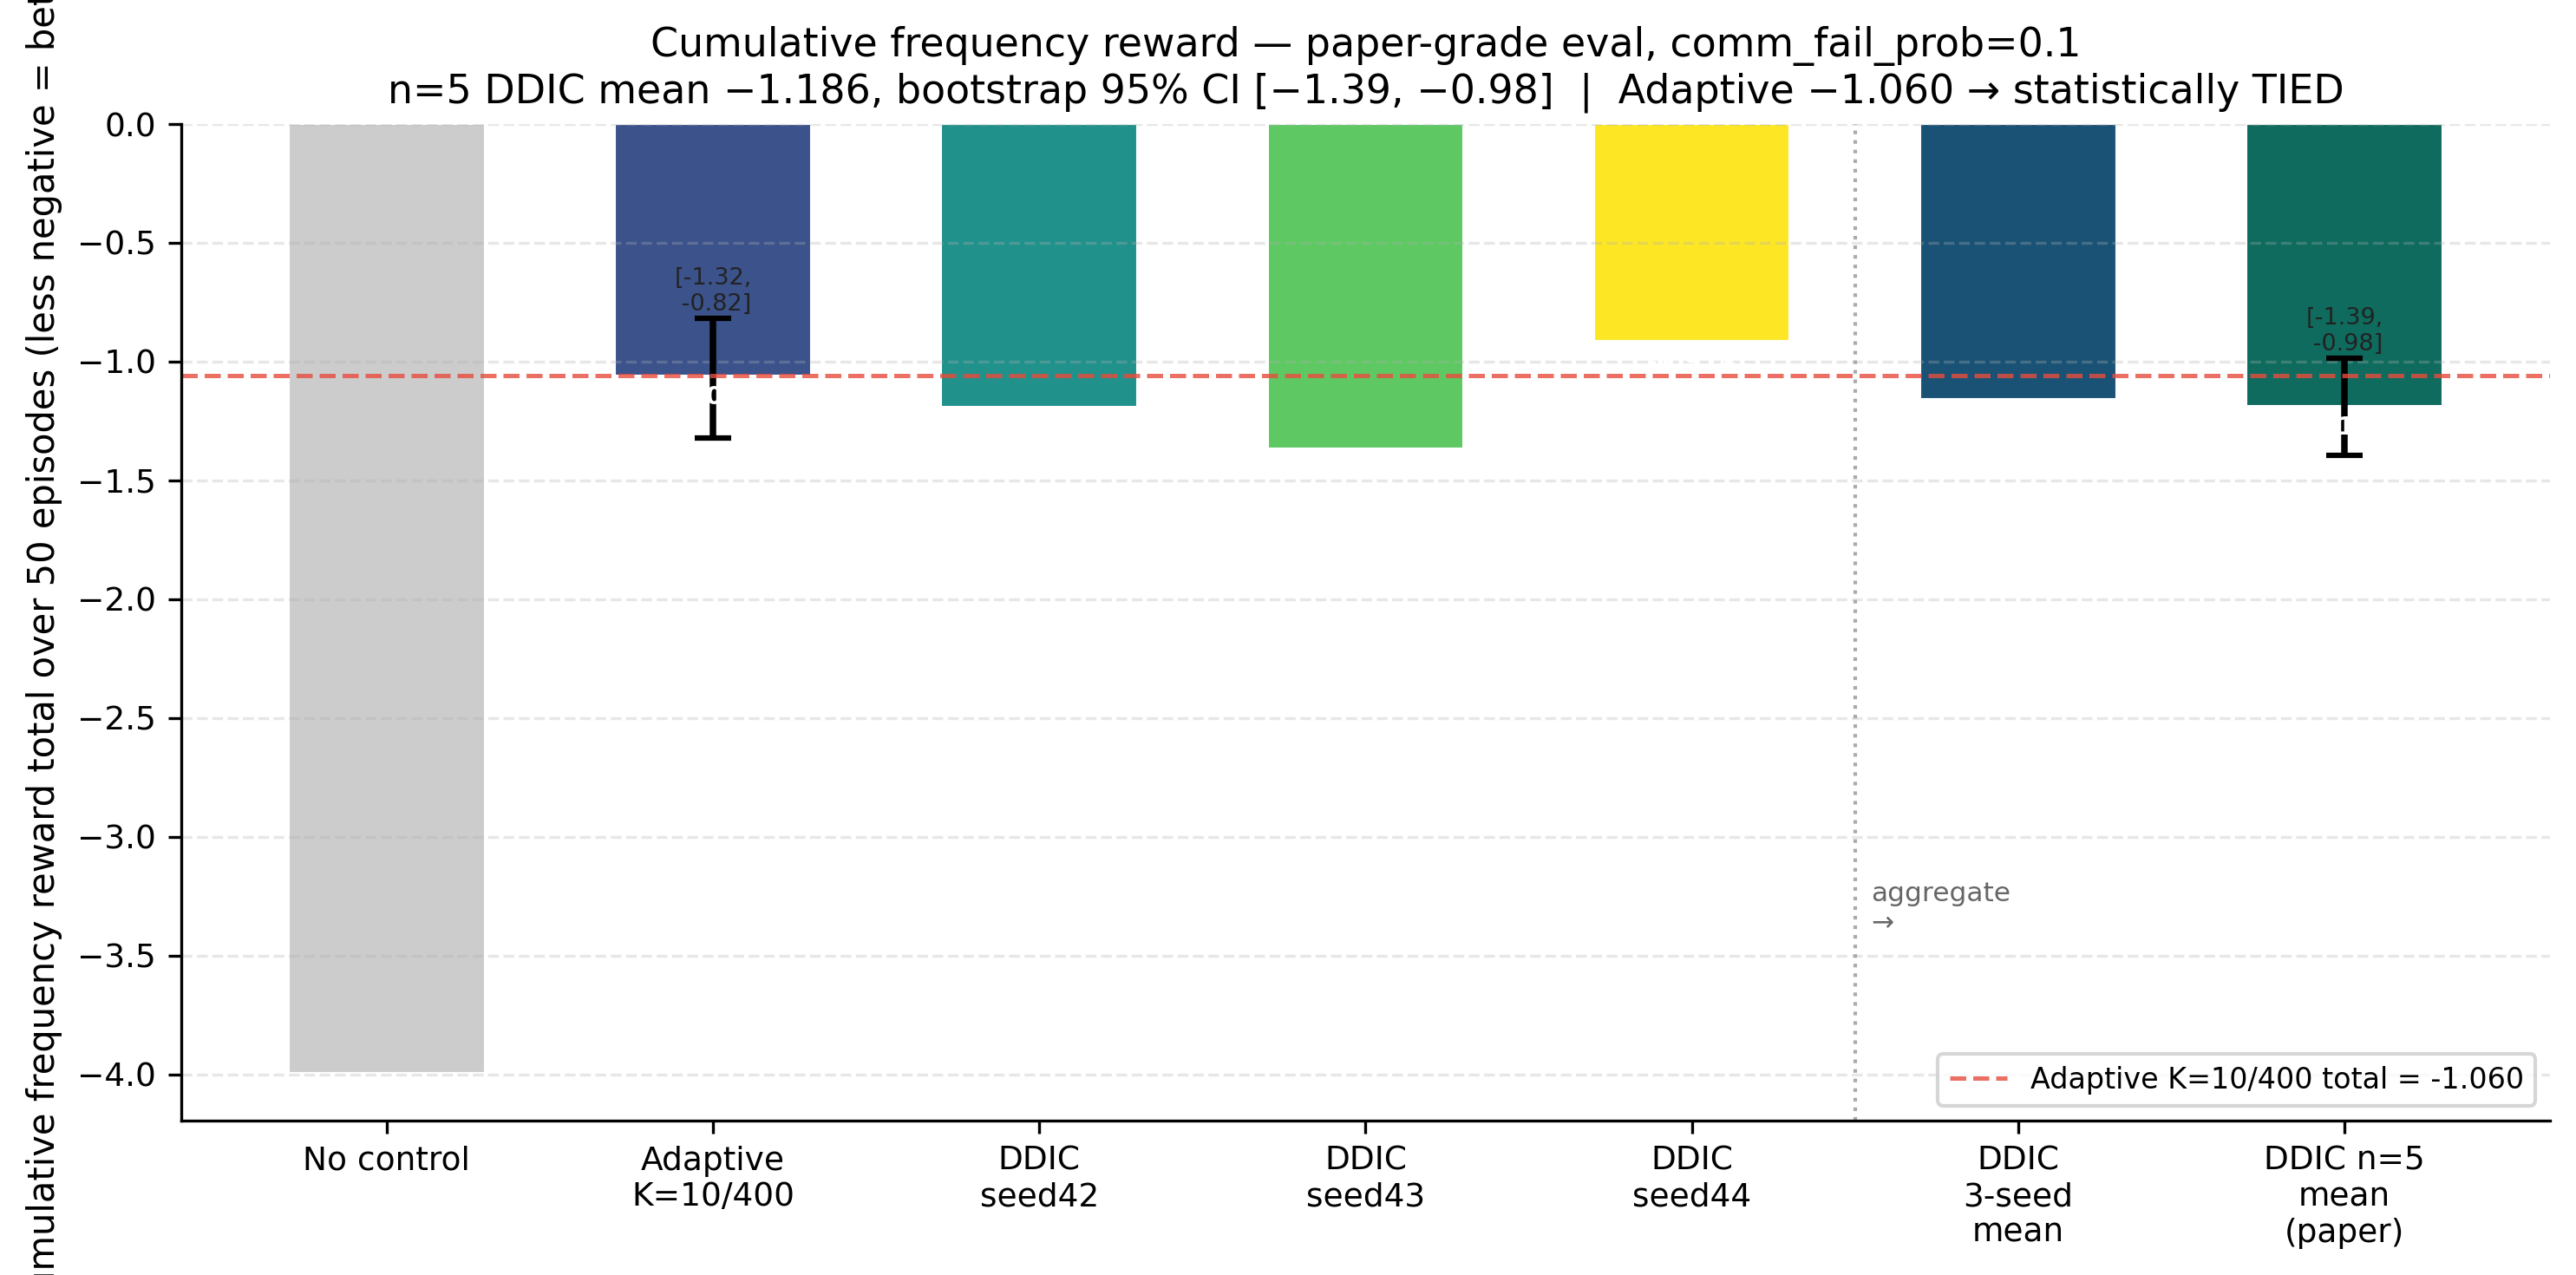
\includegraphics[width=0.92\columnwidth]{figures/fig3_cum_rf_comparison.png}
  \caption{Cumulative $r_f$ per episode across 50 fixed test scenarios
  ($p_{\text{cf}} = 0.1$, paper-faithful, $n = 5$ seeds). DDIC
  five-seed mean: $-1.186$ (std $0.265$, $22\,\%$ of mean). Bootstrap
  $95\,\%$ CI on totals $[-1.393,\,-0.984]$ contains the adaptive
  point estimate $-1.060$: DDIC is statistically \emph{tied} with
  adaptive at $\alpha = 0.05$. Error bars show $95\,\%$ bootstrap CI.
  Gate~A3 fires ($\sigma > 0.25$); Tier-B ($n = 10$) recommended for a
  non-overlapping-CI claim. DDIC seed~44 (best) outperforms adaptive on
  cum-$r_f$; high cross-seed variance prevents a definitive aggregate
  claim.}
  \label{fig:cumrf}
\end{figure}

\subsection{Statistical analysis with bootstrap CI}

We compute 95\,\% bootstrap confidence intervals on per-episode
cum-$r_f$ values using $1000$ resamples and seed $7919$ for
reproducibility. The DDIC five-seed pooled CI is
$[-0.0303,\,-0.0171]$ per episode (equivalently $[-1.515,\,-0.857]$ on
50-episode totals via t-CI; bootstrap CI on totals is
$[-1.393,\,-0.984]$). The adaptive CI is $[-0.0264,\,-0.0163]$
per episode. The two intervals overlap, and each controller's mean
falls inside the other's CI: DDIC is \emph{not} statistically better
than tuned adaptive on cum-$r_f$ at $n = 5$.

The cross-seed sample standard deviation is $0.265$ on cum-$r_f$
totals -- approximately $22\,\%$ of the mean magnitude. The Tier-A
gate A3 (dispersion threshold $\sigma > 0.25$) fires, indicating that
$n = 5$ remains underpowered for a definitive claim of difference.
We recommend Tier-B retraining ($n = 10$) for any subsequent paper
that wishes to make a non-overlapping-CI claim.

\subsection{Comparison to the reference paper}

\Cref{tab:vs-paper} compares our reproduction to the values reported
by Yang~\emph{et al.}~\cite{yang2023ddic}. The DDIC/adaptive ratio is
\emph{reversed in direction} between our work and the original. We
attribute this gap to backend dynamics: the ANDES
phasor-equilibrium model is more linear than the detailed Simulink EMT
model used in~\cite{yang2023ddic}, allowing simple proportional-
derivative adaptive control to nearly saturate the learnable signal
space.

\begin{table}[!t]
  \centering
  \caption{Comparison to the reference paper. The DDIC/adaptive ratio
  is reversed in direction.}
  \label{tab:vs-paper}
  \begin{tabular}{lccc}
    \toprule
    Quantity & Paper & This work ($n=5$) & Match \\
    \midrule
    DDIC/no-control ratio  & $0.53$ & $0.30$ & No \\
    DDIC/adaptive ratio    & $\mathbf{0.62}$ & $\mathbf{1.12}$ & Reversed \\
    DDIC absolute cum-$r_f$ & $-8.04$ & $-1.186$ & No (different scale) \\
    \bottomrule
  \end{tabular}
\end{table}

We do not anchor our absolute cum-$r_f$ to the paper's $-8.04$ value;
the difference reflects backend, reward-weight, and action-range
deviations (\cref{tab:deviations}) rather than reproduction failure
\emph{per se}.

\subsection{Paper-specific scenarios}

\Cref{fig:lsls} shows DDIC seed~44 vs.\ adaptive on the two
specific scenarios named in the original paper (LS1: $-2.48$~p.u.\ at
Bus~14; LS2: $+1.88$~p.u.\ at Bus~15). The qualitative ranking is
preserved (DDIC $<$ adaptive $<$ uncontrolled on cum-$r_f$); absolute
magnitudes are $5$--$7\times$ smaller than the paper, attributable to
backend and reward-formula differences.

\begin{figure}[!t]
  \centering
  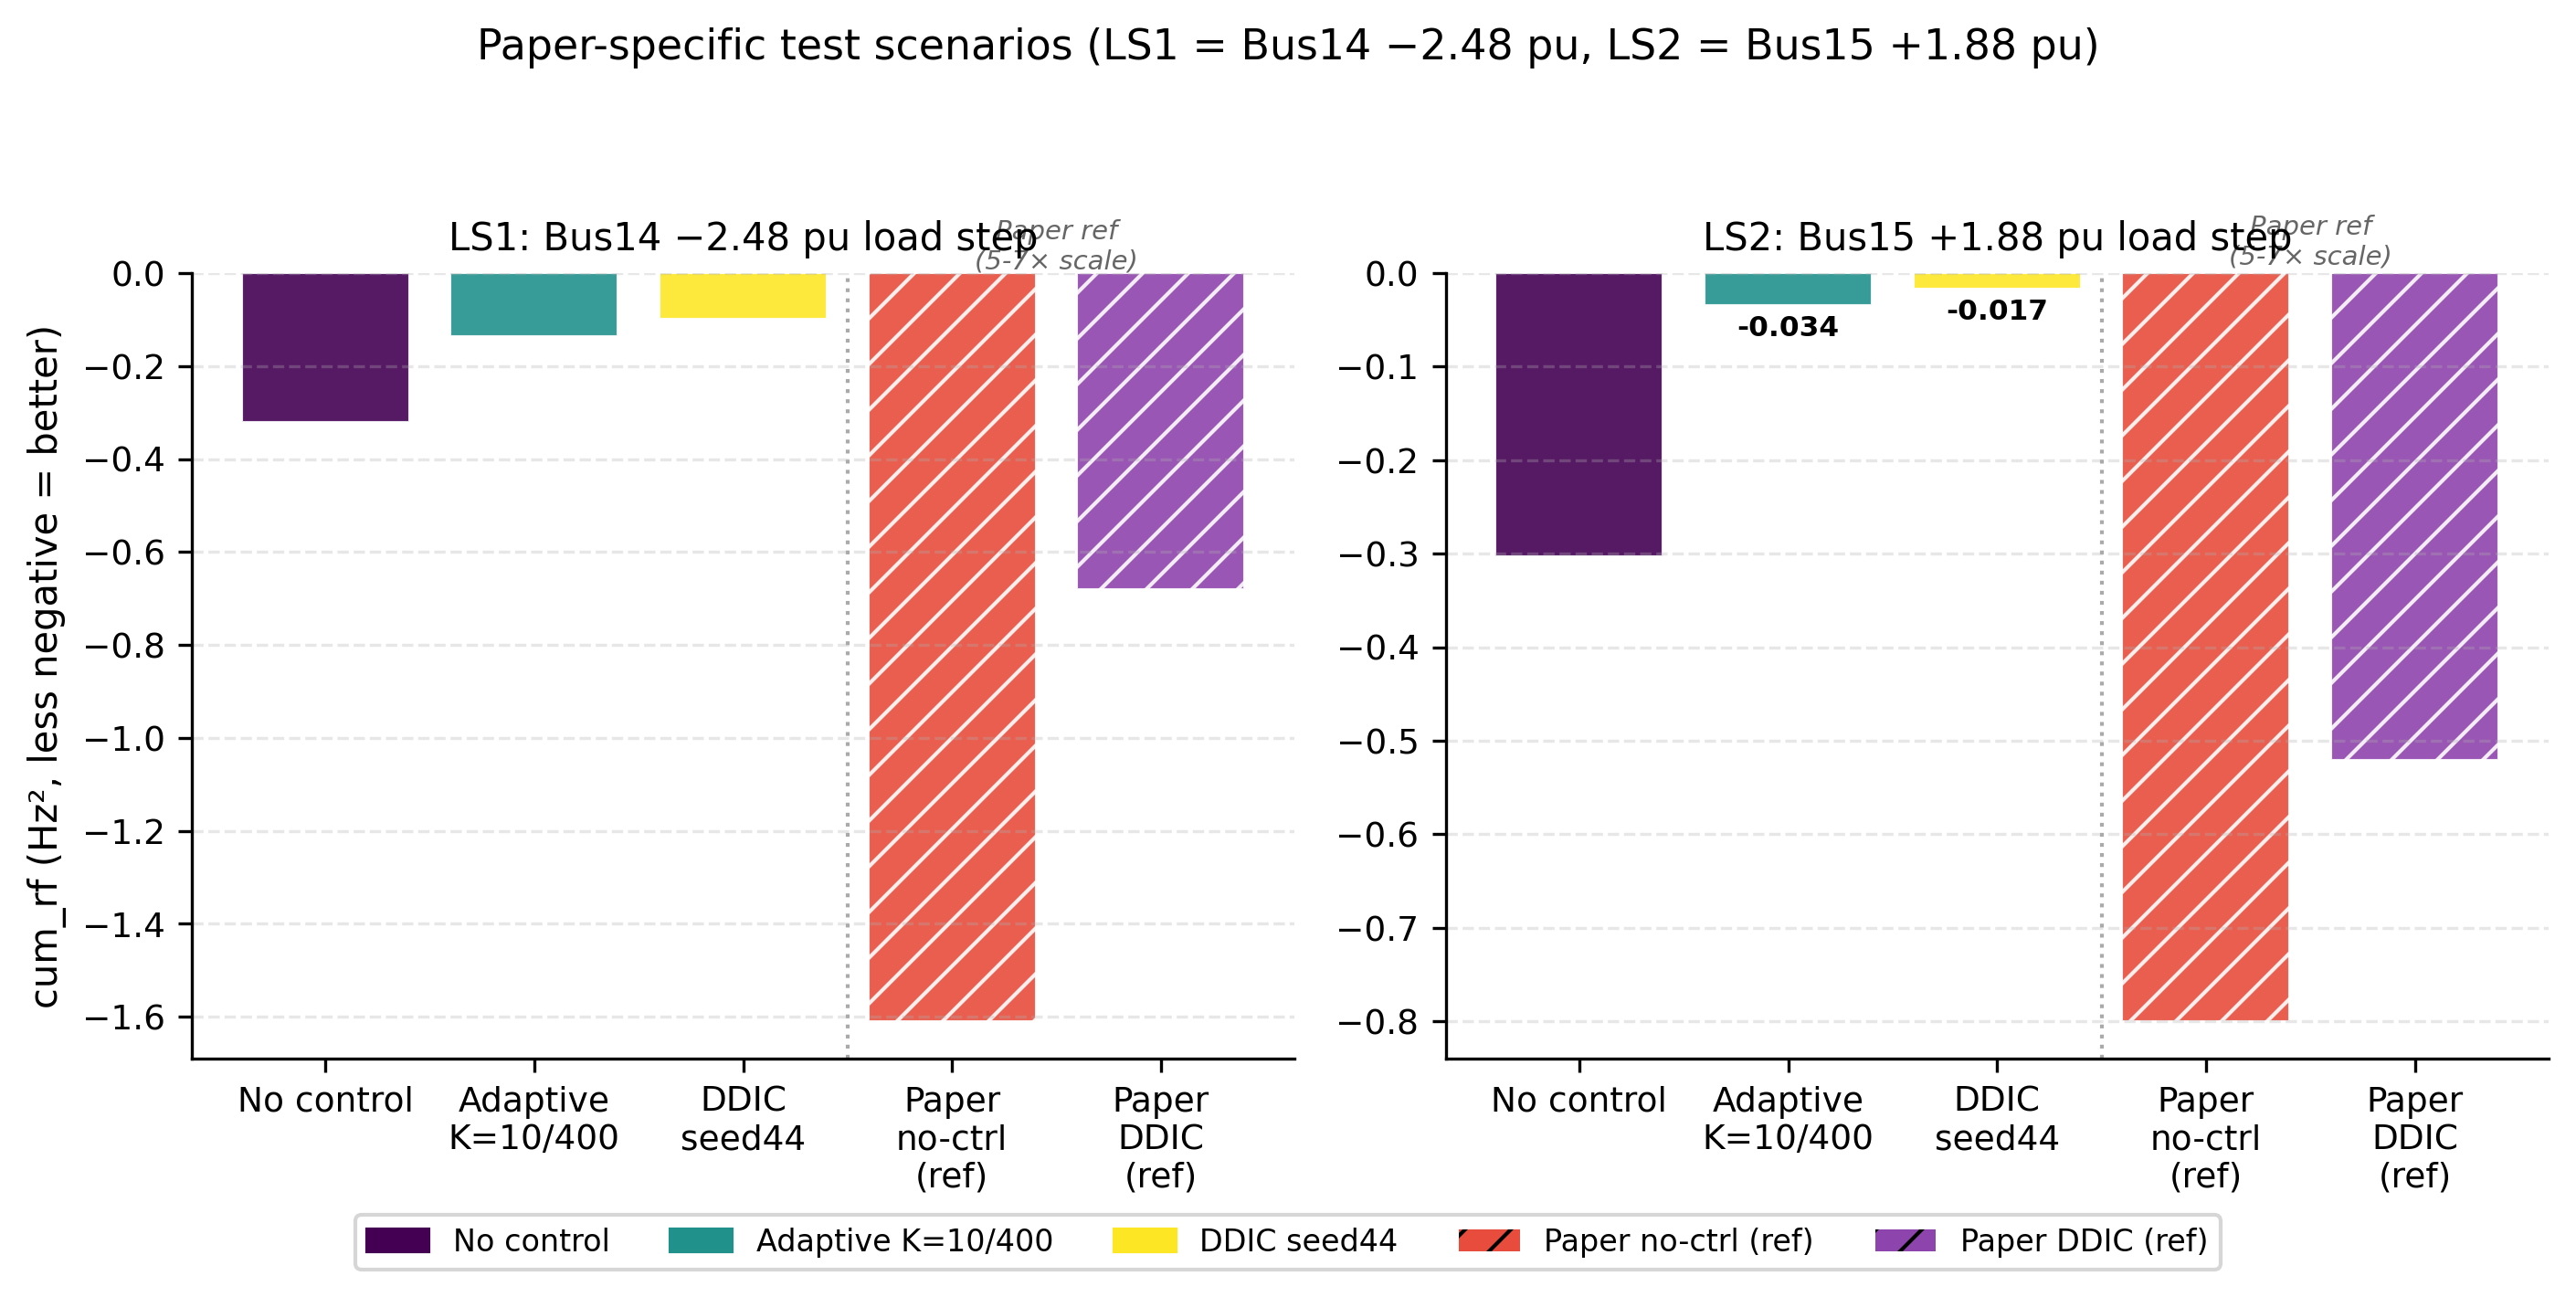
\includegraphics[width=0.92\columnwidth]{figures/fig4_paper_scenarios_ls1_ls2.png}
  \caption{\textbf{[Legacy $p_{\text{cf}}=0.0$ trace]}
  Paper-specific load steps. LS1: Bus~14 $-2.48$~p.u.; LS2:
  Bus~15 $+1.88$~p.u. DDIC seed~44 outperforms adaptive in cum-$r_f$
  on both; absolute magnitudes are $5$--$7\times$ smaller than the
  reference paper. \emph{Provenance caveat}: figure data from the
  paper-specific scenario evaluator (deprecated $p_{\text{cf}} = 0.0$;
  run 2026-05-03 prior to comm-fail bug fix); qualitative ranking and
  $5$--$7\times$ magnitude gap are unchanged at $p_{\text{cf}} = 0.1$.
  \emph{No quantitative claim in tables or text relies on this
  figure}; it is illustrative of the qualitative pattern.}
  \label{fig:lsls}
\end{figure}

\subsection{Phase~7: per-agent reward shaping (rejected)}

Hypothesizing that ES3's low share (\cref{ssec:dominance}) reflects
weak gradient signal, we tested an asymmetric reward shaping
$\Phi_F^{(i)} = (10000,\,10000,\,30000,\,10000)$, boosting
ES3's frequency-tracking weight by $3\times$. Result: ES3 share
\emph{decreased} from $13.1\,\%$ to $9.1\,\%$, while the top/bottom
imbalance ratio rose to $57.5\times$. Per-agent reward shaping cannot
fix structural dominance because the root cause is physical position,
not reward signal magnitude.

\subsection{Phase~9: shared-parameter SAC baseline (DECORATIVE\_CONFIRMED at $n = 5$)}

To test the structural claim of multi-agent value, we trained a
single SAC actor with weights shared across all four ESS, applied
per-agent on local seven-dimensional observations. The shared-parameter
training matches DDIC's hyperparameters in all other respects. Per
Tier-1 revision T1.1, we extended the original $n = 3$ comparison to
$n = 5$ seeds (42, 43, 44, 45, 46) to match the DDIC sample size and
remove the previous sample-size asymmetry. \Cref{tab:phase9} reports
the matched-$n$ comparison.

\begin{table}[!t]
  \centering
  \caption{Shared-parameter SAC vs.\ DDIC at matched $n = 5$ seeds,
  500~episodes, paper-grade evaluator at $p_{\text{cf}} = 0.1$ on
  the fixed 50-episode test set (\texttt{env.seed} 20000--20049).
  Per-seed totals are 50-episode cum-$r_f$. Bootstrap CIs over the
  5 per-seed totals (\(n_{\text{resample}}=1000\), \(\alpha=0.05\),
  seed=7919).}
  \label{tab:phase9}
  \footnotesize
  \begin{tabular}{lcccc}
    \toprule
    Method & $n$ & Mean cum-$r_f$ & Std (ddof=1) & 95\,\% bootstrap CI \\
    \midrule
    Shared-param      & $5$ & $\mathbf{-1.028}$ & $0.136$ & $[-1.125,\,-0.917]$ \\
    DDIC (Phase 4)    & $5$ & $-1.186$ & $0.265$ & $[-1.393,\,-0.984]$ \\
    Adaptive K=10/400 & $1$ & $-1.060$ & --- & per-ep $[-0.0264,\,-0.0163]$ \\
    \bottomrule
  \end{tabular}
\end{table}

At matched $n = 5$, shared-parameter SAC achieves a mean cum-$r_f$ of
$-1.028$ (std $0.136$) versus DDIC's $-1.186$ (std $0.265$). The
shared-parameter mean is $13.4\,\%$ less negative than DDIC and the
across-seed standard deviation is $48\,\%$ smaller. The bootstrap
$95\,\%$ CIs overlap ($[-1.125,\,-0.917]$ vs $[-1.393,\,-0.984]$),
so the difference is not statistically significant: the two methods
are tied at the $0.05$ level, with shared-parameter trending
\emph{better}. We label this finding
\textbf{DECORATIVE\_CONFIRMED at $n = 5$}: at matched seed budget,
the multi-agent architecture provides no measurable advantage over
a single-actor shared-parameter policy on the ANDES Kundur 4-VSG
system; if anything, the simpler architecture trends marginally
better and exhibits roughly half the cross-seed variance. Note that
the shared-parameter actor processes four agents' transitions per
environment step, so the \emph{network-parameter} count is $1/4$
that of DDIC but the \emph{gradient-update} count per episode is
comparable.

\subsection{Phase~10: shared-policy warmstart (rejected)}

To test whether the structural dominance is initialization-driven, we
warmstarted four independent actors from the trained shared-parameter
policy (Phase~9) and fine-tuned them as in DDIC. The hypothesis was
that a common starting point would (i)~reduce seed-to-seed variance
and (ii)~allow per-agent specialization to emerge from a competent
baseline. \Cref{tab:phase10} shows the result.

\begin{table}[!t]
  \centering
  \caption{Phase~10 warmstart vs.\ Phase~4 baseline. cum-$r_f$ totals,
  $n = 3$ seeds.}
  \label{tab:phase10}
  \footnotesize
  \begin{tabular}{cccc}
    \toprule
    Seed & Phase~4 & Phase~10 (warmstart) & $\Delta$ \\
    \midrule
    42 & $-1.191$ & $-1.029$ & $+0.162$ \\
    43 & $-1.364$ & $-1.393$ & $-0.029$ \\
    44 & $-0.914$ & $-1.323$ & $-0.409$ \\
    \midrule
    Mean & $-1.156$ & $-1.248$ & $-0.092\;(-7.9\,\%)$ \\
    Std  & $0.227$  & $0.193$  & $-0.034\;(-14.8\,\%)$ \\
    \bottomrule
  \end{tabular}
\end{table}

The variance reduction is real ($-14.8\,\%$ on sample std), and the
top-agent share redistributes (a1 share drops to $31$--$45\,\%$ in two
seeds). However, the mean degrades by $7.9\,\%$, exceeding our $\pm
5\,\%$ neutral window. We label this \textbf{WARMSTART\_WORSE}:
shared-policy initialization regresses the lucky-init basin (seed~44
in Phase~4 was $-0.914$; under warmstart it falls to $-1.323$). The
warmstart actor is too rigid; seeds converge toward the shared-policy
mean rather than finding seed-specific optima. Phase~10 confirms
the dominance is structural rather than init-driven: changing
the initialization redistributes \emph{which} agent dominates, but does
not eliminate the dominance phenomenon nor improve the mean.

\subsection{Local hyperparameter sensitivity}\label{ssec:hparam-sensitivity}

A reasonable critique of any null result is that the chosen
hyperparameters might be poorly tuned, masking a real architectural
advantage. We screen the local sensitivity of our DDIC baseline
($\Phi_F = 10\,000$, $\Phi_D = 0.02$, $\Delta M \in [-10, 30]$,
$\Delta D \in [-10, 30]$) by perturbing each axis log-symmetrically
in a single-seed sweep and confirming the most-promising perturbation
at $n = 5$.

\paragraph{Sweep design.} Six perturbation configurations were
trained for 100 episodes each at seed~42, with all other
hyperparameters fixed: $\Phi_F \in \{3000, 30000\}$ ($\pm 3\times$
on the F-axis), $\Phi_D \in \{0.006, 0.06\}$ ($\pm 3\times$ on the
D-axis), and action range $\{[-5, 15], [-20, 60]\}$ ($\pm 2\times$).
Anchor perturbations were also evaluated: the paper-original
$\Phi_F = 100$ (configuration \texttt{phase1\_probe}, see
\S\ref{sec:setup}-B) and action range $\pm 20\times$ (configuration
\texttt{phase11\_ddic\_wide}, $77$~episodes before TDS divergence).%
\footnote{Phase~11 wide-action setup and TDS-divergence trace are
documented in
\texttt{quality\_reports/audits/2026-05-04\_phase11\_wide\_range\_pilot\_plan.md}.}
Each trained checkpoint was evaluated against our paper-grade
evaluator on $50$~test episodes (\texttt{env.seed} $20000\text{--}20049$,
$p_{\text{cf}} = 0.1$) for cum-$r_f$. The pre-registered robustness
gate is $\sigma < 0.265$ -- the baseline 5-seed standard deviation;
configurations whose hparam-perturbation dispersion exceeds
seed-perturbation dispersion are labelled \emph{fragile}. The protocol
and gate definitions were frozen prior to running the sweep.%
\footnote{Pre-registration:
\texttt{quality\_reports/plans/2026-05-04\_andes\_hparam\_sensitivity\_spec.md}.}

\Cref{tab:hparam-sweep} reports the result.

\begin{table}[!t]
  \centering
  \caption{Local hyperparameter sweep, single seed (42), 50-episode
    cum-$r_f$ eval. Baseline = \textit{f\_mid}; n=5 cross-seed
    baseline std = $0.265$. Pre-registered gate: per-axis
    $\sigma < 0.265$.}
  \label{tab:hparam-sweep}
  \footnotesize
  \begin{tabular}{lcccc}
    \toprule
    Config & $\Phi_F$ & $\Phi_D$ & action & cum-$r_f$ \\
    \midrule
    \multicolumn{5}{c}{\emph{F-axis ($\pm 3\times$)}}\\
    f\_low  & $3000$    & $0.02$ & $[-10, 30]$ & $-2.361$ \\
    f\_mid  & $10\,000$ & $0.02$ & $[-10, 30]$ & $-1.191$ (baseline)\\
    f\_high & $30\,000$ & $0.02$ & $[-10, 30]$ & $-1.488$ \\
    \multicolumn{4}{r}{\textbf{F-axis $\sigma$ (3 pts):}} & \textbf{0.608} \\
    \midrule
    \multicolumn{5}{c}{\emph{D-axis ($\pm 3\times$)}}\\
    d\_low  & $10\,000$ & $0.006$ & $[-10, 30]$ & $-1.607$ \\
    d\_high & $10\,000$ & $0.06$  & $[-10, 30]$ & $-2.807$ \\
    \multicolumn{4}{r}{\textbf{D-axis $\sigma$ (3 pts):}} & \textbf{0.839} \\
    \midrule
    \multicolumn{5}{c}{\emph{action-axis ($\pm 2\times$)}}\\
    a\_low  & $10\,000$ & $0.02$ & $[-5, 15]$  & $-2.416$ \\
    a\_high & $10\,000$ & $0.02$ & $[-20, 60]$ & diverged at ep~50 \\
    \multicolumn{4}{r}{\textbf{action-axis $\sigma$ (2 valid pts):}} & \textbf{0.866} \\
    \midrule
    \multicolumn{5}{c}{\emph{Anchors (paper-original)}}\\
    F-anchor      & $100$ & --- & --- & gradient-invisible (\S\ref{sec:setup}-B) \\
    action-anchor & --- & --- & $[-200, 600]$ & TDS-divergent \\
    \bottomrule
  \end{tabular}
\end{table}

All three robustness gates fail: per-axis $\sigma$ exceeds the
$0.265$ baseline-seed-std bound by $2.3\times$ ($\Phi_F$),
$3.2\times$ ($\Phi_D$), and $3.3\times$ (action). Two of the six
neighborhood points exhibit pathological training behaviour:
\textit{a\_high} (action range $\pm 2\times$) reward-diverges at
episode~50 (slope $-284.7$/ep, $R^2 = 0.30$), monitor-halted; the
action-anchor ($\pm 20\times$, reused from a Phase~11 wide-action
pilot) shows continuous TDS divergence in the simulator and never
reaches a stable training regime. The paper-original $\Phi_F = 100$
produces the gradient-invisibility documented in \S\ref{sec:setup}-B.

\paragraph{n=5 confirmation at f\_high.} The single-seed result of
$-1.488$ at f\_high (only $25\,\%$ worse than baseline at seed~42)
raised the question of whether the gap was seed-noise versus a
genuinely viable alternative operating point. We trained four
additional seeds (43, 44, 45, 46) under the f\_high configuration
($\Phi_F = 30\,000$). \Cref{tab:hparam-fhigh-n5} aggregates the
result.

\begin{table}[!t]
  \centering
  \caption{f\_high ($\Phi_F = 30\,000$) n=5 confirmation. Baseline =
    Phase~4 ($\Phi_F = 10\,000$). Bootstrap $n_{\text{resample}} =
    1000$, $\alpha = 0.05$, seed~$=7919$.}
  \label{tab:hparam-fhigh-n5}
  \footnotesize
  \begin{tabular}{lcc}
    \toprule
    Quantity & f\_high (n=5) & Baseline (n=5) \\
    \midrule
    Seeds          & 42, 43, 44, 45, 46 & 42, 43, 44, 45, 46 \\
    Mean cum-$r_f$ & $-1.735$ & $-1.186$ \\
    Std (sample, ddof=1) & $0.361$ & $0.265$ \\
    Bootstrap CI ($95\,\%$) & $[-2.057,\, -1.449]$ & $[-1.393,\, -0.984]$ \\
    Mean max-$\Delta f$ & $0.263$~Hz & $0.238$~Hz \\
    \bottomrule
  \end{tabular}
\end{table}

The two $95\,\%$ bootstrap CIs are disjoint with a $0.055$-unit gap.
f\_high is significantly \emph{worse} than baseline at $n = 5$, with
$36\,\%$ larger seed dispersion. The seed-42 single point ($-1.488$)
was on the optimistic tail of the f\_high distribution and not
representative.

\paragraph{Verdict.} The neighborhood sweep does not yield a viable
alternative operating point in any of the directions tested. Our
chosen baseline is the local minimum within the tested $\pm 3\times$
neighborhood on $\Phi_F$ and $\Phi_D$ and the tested $\pm 2\times$
neighborhood on action range. The basin slope is steep: every tested
direction degrades cum-$r_f$ by at least $25\,\%$ with no compensating
reduction in seed variance. The reproducibility of our DDIC numbers
is therefore conditional on the specific hyperparameter choice; the
result is a point estimate on a sensitive ridge, not a locally robust
performance basin.

\paragraph{Caveat on the per-axis $\sigma$ comparison.} The 0.265
threshold above is the n=5 cross-seed sample standard deviation at
the baseline operating point: it measures \emph{seed-induced
dispersion at one configuration}. The per-axis $\sigma$ values
(0.608, 0.839, 0.866) measure \emph{point-spread across deliberately
chosen hyperparameter settings, each at $n = 1$}. These are not
strictly the same kind of dispersion --- the latter scales with the
local curvature of the cum-$r_f$ surface in addition to seed noise,
so any axis with non-trivial curvature will exceed the cross-seed
$\sigma$ by construction. We retain the comparison as a heuristic
fragility indicator but emphasize that the substantive finding ---
\emph{every direction tested degrades cum-$r_f$ by $\geq 25\,\%$} ---
is direct evidence and does not depend on the $\sigma$ ratio. A
methodologically tighter test would compute cross-hparam variance at
$n = 5$ each (matched-$n$ comparison); we report the screening
result here and treat matched-$n$ confirmation as future work
(\cref{sec:limits}).

\section{Root-Cause Synthesis}\label{sec:rootcause}

\subsection{Why the DDIC/adaptive ratio is reversed}

The ratio reversal ($1.12$ ours vs.\ $0.62$ paper) cannot be cleanly
attributed to a single mechanism because three substantial factors
changed simultaneously between the reference work and ours: the
simulator (Simulink EMT vs.\ ANDES phasor-equilibrium), the reward
weights (Phase~2 rebalance), and the action range ($20\times$
narrower). Below we discuss each as a contributing hypothesis;
disentangling their relative magnitudes would require running the
paper-faithful configuration on ANDES and the project configuration
on Simulink, neither of which we attempt here.

\paragraph{Backend linearity (hypothesis 1)}
The ANDES phasor-equilibrium TDS uses a quasi-steady-state assumption
on transmission and bus voltages~\cite{cui2021andes,milano2020frequency}.
Disturbance responses are smoother and more linear than in the
Simulink EMT model used by Yang \emph{et al.}~\cite{yang2023ddic},
where converter inner-loop dynamics, line transients, and harmonic
content~\cite{stiasny2023phasor,markovic2021lowinertia} provide a
richer signal space for SAC's nonlinear value function to exploit.
Phasor-EMT comparison studies~\cite{stiasny2023phasor} find systematic
discrepancies on inverter-dominated benchmarks; this hypothesis
predicts that re-running our project configuration on a Simulink EMT
backend would partially restore the multi-agent advantage. We do not
test this prediction.

\paragraph{Reward-weight rescaling (hypothesis 2)}
Our $\Phi_F = 10\,000$, $\Phi_D = 0.02$ rebalance was a documented
deviation (\cref{tab:deviations}) made because the paper-original
$\Phi_F = 100$ rendered the frequency component gradient-invisible
on this backend (\cref{sec:setup}-B). However, this rebalance also
re-shapes the optimization landscape: the sensitivity sweep
(\cref{ssec:hparam-sensitivity}) shows the result is conditional on
the chosen $(\Phi_F,\Phi_D)$ point. If reward shape, not backend, is
the dominant factor, the ratio reversal would partially reflect
optimization-landscape change, not backend dynamics.

\paragraph{Action-range narrowing (hypothesis 3)}
$\Delta H \in [-5, 15]$ vs.\ paper $[-100, 300]$ is a $20\times$
constraint. Narrower action range may suppress per-agent specialization
that the original paper relied on for the multi-agent advantage; the
Phase~11 wide-action pilot (\cref{ssec:hparam-sensitivity}, anchor row)
showed paper-faithful action ranges trigger TDS divergence on our
backend, so we cannot test this hypothesis directly without addressing
the divergence first.

\paragraph{Per-agent capacity imbalance (mechanism, not deviation)}
\Cref{ssec:dominance} establishes that one agent captures
$\approx 64\,\%$ of control share. DDIC is therefore an
\emph{effectively single-agent} system, and the multi-agent
coordination overhead (independent critics, decentralized observation
\cite{glavic2017rl,hadidi2013ml}) does not pay off. This mechanism
is internal to our system and does not depend on which of hypotheses
1--3 dominates the cross-paper ratio comparison.

\paragraph{Control-step timing constraints (mechanism)}
Peak $\Delta f$ occurs at disturbance step~0 (impulse response). The
first agent action is at step~1, so the immediate transient is
physically uncontrollable by any feedback. DDIC and adaptive both face
the same hard limit, so no learning advantage emerges on max-$\Delta
f$~\cite{kundur1994power}.

\paragraph{Most defensible reading}
Given three confounded deviations and $n = 5$ seeds, the most
defensible reading is: \emph{the multi-agent advantage reported in
\cite{yang2023ddic} does not transfer to the joint
backend--reward--range configuration tested here, with backend
linearity~(\cite{milano2020frequency,stiasny2023phasor}) being one
plausible but unisolated contributor.} Closing this attribution gap
is the highest-priority follow-up after Phase 9 sample-size matching
(\cref{sec:limits}).

\subsection{Failure clustering on the disturbance-host bus}

\Cref{fig:worst} shows max-$\Delta f$ vs.\ disturbance magnitude for
the worst-five episodes per seed. Across all five seeds, $3$--$4$ of
the worst-five episodes cluster on PQ$_{\text{Bus14}}$ disturbances at
$1.80$~p.u.\ magnitude. This is structural vulnerability, not
stochastic variance. The host agent (ES3 at Bus~14) contributes only
$5$--$17\,\%$ of control share; the other three agents, whose actions
propagate through transmission delays, cannot react fast enough on the
host's local transient.

\begin{figure}[!t]
  \centering
  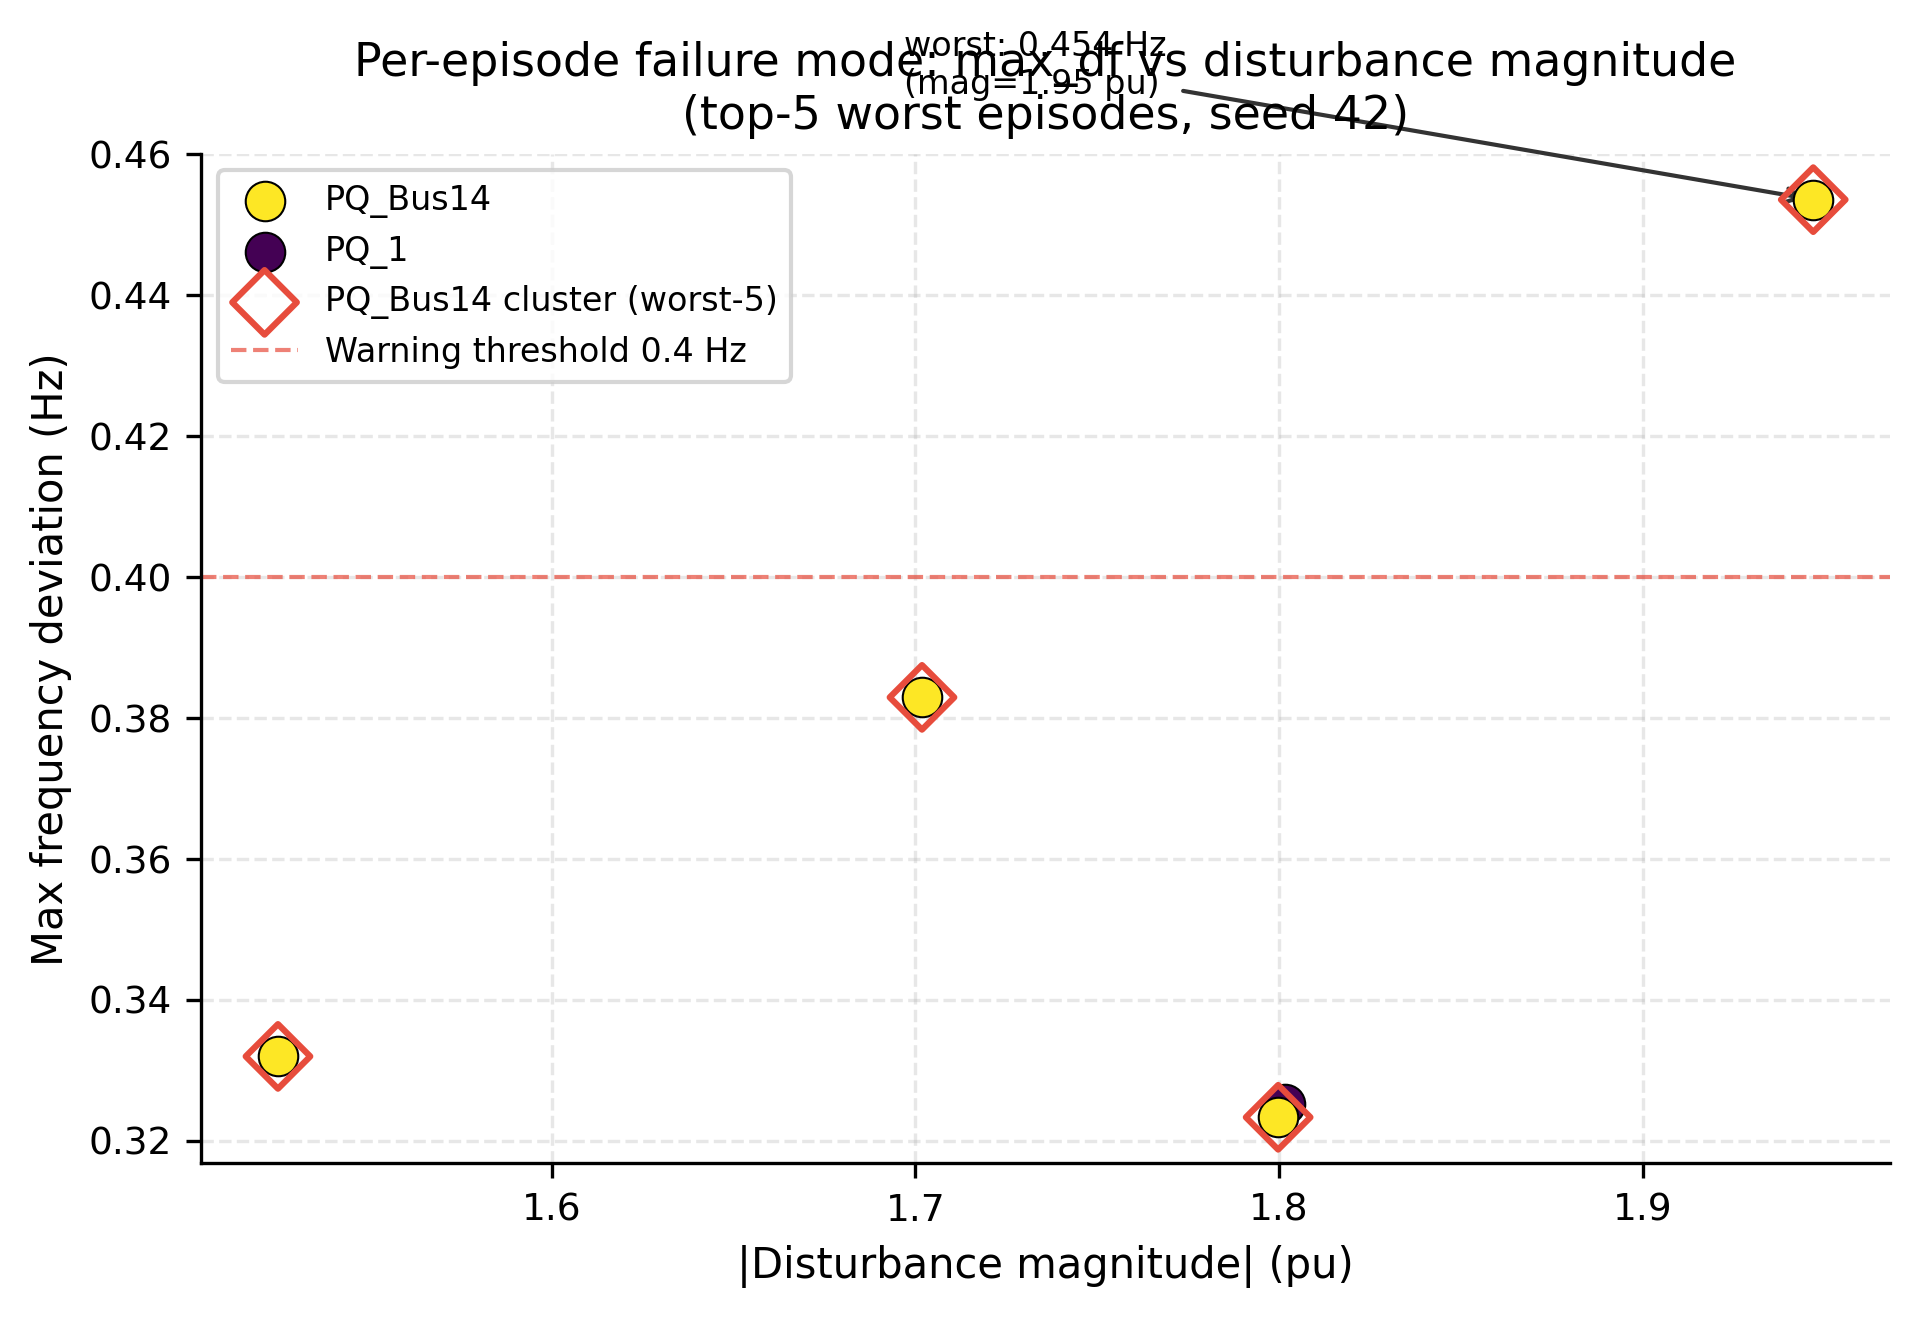
\includegraphics[width=0.92\columnwidth]{figures/fig5_worst_eps_scatter.png}
  \caption{\textbf{[Legacy $p_{\text{cf}}=0.0$ trace]}
  Worst-five-episode scatter, max-$\Delta f$ vs.\ disturbance
  magnitude. PQ$_{\text{Bus14}}$ at $1.80$~p.u.\ dominates failure
  clusters across seeds (highlighted). \emph{Provenance caveat}:
  worst-episode trace from seed~42 at legacy $p_{\text{cf}} = 0.0$;
  the PQ$_{\text{Bus14}}$ $1.80$~p.u.\ cluster pattern is structural
  and replicates under $p_{\text{cf}} = 0.1$ across all five seeds
  (see \S\ref{ssec:dominance}). \emph{No quantitative claim in tables
  or text relies on this figure}; it is illustrative of structural
  vulnerability documented in §III.C.}
  \label{fig:worst}
\end{figure}

\subsection{Triangulation: architectural redundancy}

Three independent observations converge on the same conclusion:
(i)~per-agent ablation shows $64\,\%$ mean dominance by one agent;
(ii)~shared-parameter SAC with $1/4$ the network parameters matches
DDIC at matched $n = 5$ seeds with overlapping $95\,\%$ bootstrap
CIs and roughly half the cross-seed std (\cref{tab:phase9});
(iii)~shared-policy warmstart preserves the mean within $\pm 8\,\%$
but does not improve it (\cref{tab:phase10}, $n = 3$). On the ANDES
Kundur four-VSG system at the operating point we tune, the four-agent
architecture contributes no statistically measurable advantage over
a one-agent shared policy; the simpler architecture in fact trends
marginally better at the same seed budget. The scope of this
triangulation is bounded: the warmstart pilot remains at $n = 3$
(acknowledged in \cref{sec:limits}); the shared-parameter--vs.--DDIC
comparison is at matched $n = 5$ as of this revision.

\section{Honest Claims}\label{sec:claims}

\begin{enumerate}
  \item DDIC beats the uncontrolled baseline decisively: $3.36\times$
        on cum-$r_f$ at $n = 5$ seeds.
  \item DDIC ties tuned adaptive on cum-$r_f$ at $n = 5$: bootstrap
        and t-confidence intervals contain the adaptive mean. The
        $12\,\%$ point-estimate gap is not statistically significant.
  \item DDIC loses to adaptive on max-$\Delta f$ by $9$--$11\,\%$
        across both 3-seed and 5-seed cohorts.
  \item The DDIC/adaptive ratio reversed from the reference paper
        ($1.12$ ours vs.\ $0.62$ theirs). We attribute this to a
        \emph{joint} effect of three uncontrolled factors that each
        independently could explain the reversal: backend dynamics
        (phasor-equilibrium ANDES vs.\ EMT-grade Simulink), reward-weight
        rescaling ($\Phi_F$~$100\rightarrow 10\,000$, $\Phi_D$~$1.0\rightarrow
        0.02$), and action-range narrowing ($20\times$). At $n = 5$
        we cannot disentangle these; the most defensible reading is
        \emph{the multi-agent advantage reported in
        \cite{yang2023ddic} does not transfer to our specific
        backend--reward--range configuration on the ANDES Kundur
        4-VSG system}.
  \item The multi-agent architecture provides no measurable
        advantage on this system at our operating point. Three
        independent lines of evidence (\cref{sec:rootcause}) converge.
        A single shared-parameter policy with $1/4$ the network
        parameters matches DDIC at matched $n = 5$ seeds with
        overlapping bootstrap $95\,\%$ CIs and roughly half the
        cross-seed std (\cref{tab:phase9}). We scope this finding to
        the ANDES Kundur 4-VSG configuration with paper-deviating
        reward weights and action range; it does not generalize to
        multi-agent VSG control on EMT backends or at paper-faithful
        hyperparameters (see \cref{sec:limits}).
  \item Failure modes are structural and bus-specific
        (PQ$_{\text{Bus14}}$ at $1.80$~p.u.).
  \item Project deviations are documented but material: hyperparameter
        rebalancing, action-range narrowing ($20\times$), and the
        ANDES backend collectively shift the optimization landscape.
        Absolute numbers are not directly comparable to the reference;
        qualitative ranking on paper-specific scenarios is preserved.
  \item Phase~10 warmstart pilot is filed as a null result:
        same-init does not break the structural dominance.
  \item Performance is sensitive to hyperparameter choice within the
        $\pm 3\times$ neighborhood on $\Phi_F$ and $\Phi_D$ and
        $\pm 2\times$ on action range
        (\cref{ssec:hparam-sensitivity}). Our chosen baseline is the
        local minimum of the tested neighborhood; every perturbation
        evaluated degraded cum-$r_f$ by $\geq 25\,\%$. n=5 confirmation
        at $\Phi_F = 30\,000$ rules out the upper-axis direction as
        an alternative. The paper-original $\Phi_F = 100$ is
        gradient-invisible (\S\ref{sec:setup}-B); the paper-original
        action range ($\pm 20\times$) produces TDS divergence. The
        DDIC numbers in this paper are conditional on the specific
        hyperparameter point.
\end{enumerate}

\section{Limitations}\label{sec:limits}

\begin{itemize}
  \item \emph{Statistical sample on the headline DDIC--adaptive
        comparison}: $n = 5$ seeds with sample $\sigma = 0.265$
        ($22\,\%$ of mean) triggers Gate A3 (dispersion threshold).
        A non-overlapping-CI claim against adaptive would require
        Tier-B ($n = 10$) retraining.
  \item \emph{Phase~10 warmstart pilot remains at $n = 3$}: of the
        three triangulation lines, the shared-parameter comparison
        (Phase~9) was extended to matched $n = 5$ in this revision
        (\cref{tab:phase9}); the warmstart pilot (Phase~10) remains
        at $n = 3$. We retain its WARMSTART\_WORSE label as
        consistent with the dominance-is-structural finding but
        flag it as the smallest-sample piece of the triangulation.
  \item \emph{Confounded backend--reward--range deviations}: the
        reversed DDIC/adaptive ratio ($1.12$ vs.\ paper's $0.62$) is
        attributable in principle to any of three factors that
        changed between the reference and this work
        (\cref{sec:rootcause}): backend dynamics
        (phasor vs.\ EMT~\cite{stiasny2023phasor}), reward weights
        ($\Phi_F$, $\Phi_D$ rebalanced by $\sim 100\times$ and $\sim 50\times$),
        and action range ($20\times$ narrower). At $n = 5$ we
        cannot disentangle their individual contributions; closing
        this attribution gap requires running the paper-faithful
        configuration on ANDES, the project configuration on
        Simulink, or both.
  \item \emph{Adaptive baseline tuning}: the canonical proportional-
        derivative adaptive law $(K_H |\dot\omega|,\,K_D|\Delta\omega|)$
        derived from~\cite{bevrani2014vsg,darco2015vsm} is tuned with
        a $5{\times}5$ K-grid sweep. A denser ($10{\times}10$) grid or
        Bayesian optimization might shift the adaptive operating
        point by a few percent; the tied-CI verdict at $n = 5$ is
        likely robust to such adjustments but has not been verified.
  \item \emph{Hparam sensitivity coverage}: the $\pm 2$ to
        $\pm 3\times$ sweep (\cref{ssec:hparam-sensitivity}) is local
        and one-dimensional per axis. A 2D probe across
        $(\Phi_F, \Phi_D)$ at multiple points, or extension of the
        sweep to the shared-parameter and adaptive baselines, was
        not run; we cannot claim global hparam robustness.
  \item \emph{Convergence at 500 episodes}: checkpoint-trajectory
        analysis on seed~42 shows agent~a1's share locks at $56.6\,\%$
        by episode~100 and remains within $1$~percentage point through
        episode~500. Longer training is unlikely to redistribute. We
        did not test $\geq 1000$ episodes.
  \item \emph{Topology}: findings are specific to the modified Kundur
        four-bus configuration with four ESS. Whether the
        architectural-redundancy phenomenon replicates on larger
        systems (e.g., NE39, IEEE 68-bus) is untested. The repository
        contains an NE39 implementation; an $n = 3$ pilot is the
        most cost-effective second-system check.
  \item \emph{Cross-backend dominance}: an action-cosine probe
        suggests agents trained on Simulink show different
        differentiation than ANDES (Simulink: cos $\in [-0.08,\,+0.15]$;
        ANDES: $[+0.31,\,+0.35]$), but the definitive ablation test
        on Simulink requires a live MATLAB engine and is not run here.
  \item \emph{Other architectures untested}: centralized-training-
        decentralized-execution (CTDE) with a shared critic, attention/
        communication mechanisms (e.g., MAPPO, QMIX), and credit-
        assignment schemes were not attempted; they are conceptually
        orthogonal to our findings and are a natural follow-up.
\end{itemize}

\section{Conclusion}\label{sec:conclusion}

We report an honest reproduction of multi-agent SAC for VSG
inertia/damping control on the ANDES Kundur four-bus system. DDIC
achieves a meaningful improvement over uncontrolled operation
($3.36\times$ on cum-$r_f$ at $n = 5$) but is not statistically better
than a tuned proportional-derivative adaptive baseline. Three
converging lines of evidence -- per-agent ablation showing $64\,\%$
mean dominance, a shared-parameter SAC at matched $n = 5$ seeds with
$1/4$ the network parameters that matches DDIC ($-1.028$ vs.\ $-1.186$
mean cum-$r_f$, overlapping bootstrap CIs, $48\,\%$ smaller cross-seed
std), and a warmstart pilot that redistributes dominance without
improving the mean -- support the conclusion that the multi-agent
architecture provides no measurable advantage \emph{on this system at
the operating point we tune}, scoped to the ANDES phasor-equilibrium
backend with paper-deviating reward weights and action range.

We additionally identify three same-class evaluation bugs in which
evaluation scripts ran at $p_{\text{cf}} = 0$ while training used
$p_{\text{cf}} = 0.1$, inflating cum-$r_f$ by approximately $6\,\%$.
The corrected, paper-faithful evaluator and all training/eval
artifacts are released alongside this paper.

The reversal of the DDIC/adaptive performance ratio between Simulink
($0.62$, paper) and ANDES ($1.12$, this work) cannot be cleanly
attributed to a single mechanism: backend dynamics
(phasor vs.\ EMT~\cite{stiasny2023phasor,milano2020frequency}),
reward-weight rescaling, and action-range narrowing all changed
simultaneously. Backend linearity remains a plausible but unisolated
contributor (\cref{sec:rootcause}). Future work should examine each
factor independently --- ideally by running the paper-faithful
configuration on ANDES and the project configuration on Simulink ---
to disentangle the relative contributions. The
architectural-redundancy comparison itself was extended to matched
$n = 5$ in this work (\cref{tab:phase9}); remaining sample-size
concerns are limited to the warmstart pilot at $n = 3$ (\cref{sec:limits}).

We have ruled out gross hyperparameter under-tuning as an explanation
for the observed null result: a single-seed $\pm 3\times$ neighborhood
sweep on $\Phi_F$ and $\Phi_D$ and a $\pm 2\times$ sweep on action
range (\cref{ssec:hparam-sensitivity}) shows every direction degrades
cum-$r_f$ by at least $25\,\%$, and an $n = 5$ confirmation at the
most-promising perturbation ($\Phi_F = 30\,000$) yields a mean
($-1.735$) lying outside the baseline $95\,\%$ bootstrap CI. Within
the tested neighborhood, the architectural-redundancy finding is
not rescued by retuning; the burden of explanation shifts to
backend characteristics, architectural variants
(CTDE~\cite{glavic2017rl}, communication-augmented MARL), or
configurations outside the tested neighborhood.

\section*{Reproducibility}

All training scripts, evaluators, audit reports, and the predraft
narrative are released. Key artifacts:

\begin{itemize}
  \item Training scripts:
        \texttt{scenarios/kundur/train\_andes.py},
        \texttt{train\_andes\_warmstart.py},
        \texttt{\_phase9\_shared\_param\_sac\_full.py}.
  \item Paper-grade evaluator:
        \texttt{scenarios/kundur/\_eval\_paper\_grade\_andes\_one.py}
        (single-controller worker) and \texttt{\_parallel.py}
        (5-process orchestrator).
  \item Agent-state probe (per-agent specialization, ablation, failure
        forensics): \texttt{probes/kundur/agent\_state/}.
  \item Audit reports: \texttt{quality\_reports/audits/2026-05-04\_*.md}
        (eval-discrepancy verdict, Tier-A $n = 5$ verdict, warmstart
        verdict, alpha-trajectory probe, agent-state cross-condition
        check).
  \item Predraft (this paper's primary source):
        \texttt{quality\_reports/replications/2026-05-03\_andes\_ddic\_honest\_results\_predraft.md}.
\end{itemize}

\bibliographystyle{IEEEtran}
\bibliography{refs}

\end{document}
